% This is samplepaper.tex, a sample chapter demonstrating the
% LLNCS macro package for Springer Computer Science proceedings;
% Version 2.20 of 2017/10/04
%
\documentclass[runningheads,custombib]{llncs}
%
\usepackage{graphicx}
% Used for displaying a sample figure. If possible, figure files should
% be included in EPS format.
%
% If you use the hyperref package, please uncomment the following line
% to display URLs in blue roman font according to Springer's eBook style:
% \renewcommand\UrlFont{\color{blue}\rmfamily}

%my package
\usepackage[backend=biber,
%this is the label style in the bibliography at the end of document
style=numeric,
%this is the label style for each citation in the document
citestyle=numeric,
sorting=none,
%sortcae=false                  
%citestyle=authoryear
]{biblatex}
%\usepackage[backend=biber]{biblatex}
\addbibresource{paper.bib} %Imports bibliography file

\usepackage{amsmath}
\usepackage{amsfonts}

\usepackage{tikz}
\usetikzlibrary{chains,shapes.multipart}
\usepackage{pgf}
\usepackage{tikz}
\usetikzlibrary{arrows,automata}

\usepackage{listings}
\usepackage{color}
\usepackage{float}


%% BEGIN PRISM CODE LISTING 
\definecolor{dkgreen}{rgb}{0,0.6,0}
\definecolor{gray}{rgb}{0.5,0.5,0.5}

\lstset{frame=tb,
	language=Java,
	aboveskip=1mm,
	belowskip=1mm,
	showstringspaces=false,
	columns=flexible,
	basicstyle={\fontsize{8.8}{8.5}\ttfamily},
	numbers=none,
	numberstyle=\tiny\color{gray},
	keywordstyle=\color{blue},
	commentstyle=\color{dkgreen},
	breaklines=true,
	breakatwhitespace=true,
	tabsize=3,
	morekeywords={ctmc,event, gsmp, dirac, exponential, uniform, weibull, erlang,
		module, init, rewards, endrewards, label, true, endmodule}
}
\usepackage{csquotes}

\usepackage{hyperref}

\begin{document}
%
\title{Continuous-Time Markov Chain with Alarms analysis and comparison of tools \thanks{Thanks t}}
%
%\titlerunning{Abbreviated paper title}
% If the paper title is too long for the running head, you can set
% an abbreviated paper title here
%
\author{Thomas Mari\inst{1,2}}%\orcidID{0000-1111-2222-3333}}
%
\authorrunning{F. Author et al.}
% First names are abbreviated in the running head.
% If there are more than two authors, 'et al.' is used.
%
\institute{ENS-Rennes, Campus de Ker lann, Avenue Robert Schuman, 35170 Bruz, France \and
Masaryk University, Botanická 68A, 602 00 Brno-Královo Pole, Czech republic
\email{thomas.mari@ens-rennes.fr}\\
\url{http://perso.eleves.ens-rennes.fr/people/thomas.mari/}
}
%
\maketitle              % typeset the header of the contribution
%
\begin{abstract}
For the analysis of ACTMC, Phase-type fitting is the advised way of modeling non-Markovian distributions within PRISM model checker. We ran experimental computations and deduced a reliable way of obtaining precise analysis results for phase-type fitted PRISM CTMCs.
We aim to compare Phase-type fitting with other approaches that handle directly the non-Marlovian distributions in term of efficiency and precision.

%The abstract should briefly summarize the contents of the paper in
%150--250 words.

\keywords{PRISM model checker \and CTMC \and deterministic timeout \and phase-type distribution \and ACTMC \and modeling \and analysis.}
\end{abstract}
%
%
%
\section{Introduction}

	PRISM \cite{KNP11} and Storm \cite{DBLP:journals/corr/DehnertJK017} are popular tools for modeling and analysis of stochastic systems in continuous time. They use efficient algorithms for analysis of continuous time Markov chains (CTMC). This approach suffers from a severe restriction of expressiveness, because the time between transitions must be exponentially distributed. This restriction can be remedied by the use of phase-type distributions, which can approximate any general distribution with arbitrary accuracy by only using exponential distributions \cite{Buchholz:2014:IMP:2683922}. However, the use of phase-type distributions drastically increases the number of states within the CTMC.
	
	In this paper, we experimentally evaluate the precision of the result and required computation time of various approaches to analysis of continuous time stochastic models with deterministic transitions (timeouts). PH fitting results with PRISM are compared with the results of the models in GSMP PRISM, our extension of PRISM, capable of efficiently analyzing CTMC with non-Markovian alarms (ACTMC).
	
%	BIGGER INTRO
	


\section{Related Work}
There are various tools and models in the area of probabilistic verification, especially in the analysis of non-Markovian Model. One of those model is stochastic Petri Nets. Oris is a tool for the analysis of stochastic Petri nets \cite{Bucci2010}. Oris allows to analyze Petri net with plenty of time distributions for each event such as exponential, Dirac, Uniform or instant. The expressiveness is sufficient to work on Petri nets that are equivalent to an ACTMC. This tool compute the Steady states probability as well as well as the transient state probability which is state probability at a given time. 

A less expressive model is the CTMC defined in Subsection \ref{CTMC_def}, PRISM\cite{KNP11} and Storm \cite{DBLP:journals/corr/DehnertJK017} are both well known tools to analyze CTMC. The engine of those tools are quite efficient for analysis due to the memoryless property of the exponential distribution. Phase-type (PH) approximation can be used to approach a non-Markovian model. The downside of PH approximation is the increase of the number of states which can slow down the process of analysis.  PH Fitting can be challenging depending on the PH distribution\cite{DBLP:journals/corr/KorenciakKR14}.
There are kinds of distributions which require a lot of phases to be accurately approached by PH fitting. One of those distributions is a shifted exponential distribution, which can be seen as a sequence of a deterministic timeout and a exponential distribution. The motivation of using those distributions is to depict better some events like transmissions that can't happen immediately due to physical limits.

There are automatic tools that do the Phase-Type Fitting like HyperStar \cite{10.1007/978-3-642-40725-3_13}. The power of this tools is to work on real dataset. According the system you want to model it is indeed practical to use real data such that the model depict more precisely the system. 


An alternative of PH-approximation is to work directly with a d-CTMC which is a CTMC plus deterministic distribution. This paper \cite{DBLP:journals/corr/BaierDKKR17} depict an efficient approach to analyze ACTMC with distributions where phase-type increase significantly the number of states with reasonable precision. Those distributions are amongst shifted exponential distribution and fixed-delay distribution.

A different objective on the analysis of non-Markovian model is to synthesize optimal parameter. We can add a reward system on the model and computed the optimal parameter, like a timeout on some transitions such that the mean-payoff is $\epsilon$-optimal \cite{DBLP:journals/corr/BaierDKKR17}. The mean-payoff can be seen as the average long term efficiency of the system.


\section{Preliminaries}
We will go through the theoretical bases needed to understand the contribution. For a complete understanding you can refer to the chapter two of this thesis \cite{Korenciak2018thesis}.
\subsection{Time distribution}
The class of models we use is probabilistic continuous time model, which means that the time passed in a state will depend on a time distribution. A time distribution can be depicted by its cumulative distribution function (CDF) $F : \mathbb{R} \rightarrow[0,1]$, $F(t)$ is the probability that the event will happen before the time $t$. The exponential distribution of rate $\lambda$ has a CDF $F(t) = 1 - \exp(-\lambda t)$, it is important to keep in mind that a rate refers to the exponential distribution. The Dirac distribution of timeout $\tau$ has a CDF $F(t) = 
\left\{
	\begin{array}{l}
		0 \text{ if } t < \tau\\
		1\text{ else}
	\end{array}
\right.$. The keyword deterministic is used when referring to so event following a Dirac distribution.
The Erlang distribution can be seen as the distribution of a sequence of $k$ exponential distribution of parameter $\lambda$. Hence, the Erlang distribution has two parameter $k$ and $\lambda$. 
In this paper, time distribution which are not exponential will be called non-Markovian distribution. Hence, a non-Markovian model will refer to a model with non-Markovian distribution.
\subsection{CTMC}
\label{CTMC_def}
A continuous-time Markov chain (CTMC) is a triple $C = (S,Q,s_{in})$, where 
\begin{itemize}
	\item[$\bullet$] S is a finite set of states
	\item[$\bullet$] $Q : S \times S \rightarrow \mathbb{R}_{\geq 0}$ is a matrix of rates such that $\sum_{s' \in S} Q(s,s')  > 0$ for each $s \in S$
	\item[$\bullet$] $s_{in} \in S$ is an initial state
\end{itemize} 
$Q(s,s')$ is the rate of the transition from $s$ to $s'$.
We define the exit rate of state $s$ as $\lambda_s = \sum_{s' \in S} Q(s,s')$

A run of a CTMC $\mathcal{C}$ is an infinite alternating sequence of states and times $\omega = s_0t_0s_1t_1...$ where 
\begin{itemize}
	\item[$\bullet$] $s_0 = s_{in}$
	\item[$\bullet$] $s_i$ is the i-th state
	\item[$\bullet$] $t_i$ is the time spent in $s_i$
\end{itemize}

For each $i \in \mathbb{N}$ \begin{itemize}
	\item[$\bullet$] $t_i$ is choosen randomly according to the exponential distribution with rate $\lambda_{s_i}$
	\item[$\bullet$] $s_{i+1}$ is choosen according to the discrete distribution $\dfrac{Q(s_i,.)}{\lambda_{s_i}}$
\end{itemize}

Without considering the time spent on each state, CTMC works the same way than discrete time Markov Chain. It is interesting to understand why it is difficult to allow non-Markovian distribution. In this case, when available transitions are not exponential, we cannot pick the next state as easily. We will see an extension of CTMC, where we allow at most one non-Markovian at the same time. 

\subsection{ACTMC}

%Continuous-Time Markov Chain with Alarms (ACTMC)s. I won't give the formal semantics which might not fit in this paper. 
We can see ACTMC as CTMC with some events called alarms that are enabled in disjoints sets of states and those events has their own timer which is active only when inside the enabled set and happend according to some continuous time distribution. Those alarms work concurrently with the exponential transition seen in the CTMC.

An ACTMC $\mathcal{A}$ is a tuple $(S,Q,s_{in},A,\langle S_a \rangle,\langle P_a \rangle,\langle F_a \rangle)$
where :
\begin{itemize}
	\item[$\bullet$]$(S,Q,s_{in})$ is a CTMC
	\item[$\bullet$] $A$ is a set of alarms
	\item[$\bullet$] $\langle S_a \rangle = (S_a)_{a \in A}$, the set of states where $a$ is enabled
		\begin{itemize}
			\item[$\bullet$] if $a \neq a'$ then $S_a \bigcap S_{a'} = \emptyset$ 
		\end{itemize}
	\item[$\bullet$]$\langle P_a \rangle = (P_a)_{a \in A}$ where $P_a$ is a probability matrix
	\item[$\bullet$]$\langle F_a \rangle = (F_a)_{a \in A}$ where $F_a$ is a cumulative distribution function (CDF) 
\end{itemize}


The operational behavior of an ACTMC is the following. A run of a ACTMC $\mathcal{A}$ is an infinite alternating sequence of states and times $(s_0,\eta_0)t_0(s_1,\eta_1)t_1...$ where 
$s_i$ is the i-th state, 
$t_i$ is the delay in $s_i$, the time spent in $s_i$ and 
$\eta_i$ is the value of the timer, the remaining time for the alarm to ring.We define $S_{off} = S\setminus\bigcup_{a \in A} S_a$ the set of states where no alarms are enabled

The sequence is defined by induction on $i$. For the initialization $s_0 = s_{in}$. $\text{If } s_0 \in S_{off} \text{ then } \eta_0 =\infty \text{. If } s_0 \in S_{a}\text{, then } \eta_0 \text{ is randomly choosen according to }F_a$. For each $i \in \mathbb{N}, t_i$ is choosen randomly according to the exponential distribution $\lambda_{s_i}$. This value might be overwritten during the induction.

Considering the induction, two cases are possible, either the alarm ring ($\eta_i \leq t_i$) or $t_i$ is too short and the alarm doesn't ring.

%CASE 1
If $\eta_i \leq t_i$, the alarm ring. 
$t_i := \eta_i$ the value of delay is overwritten and match the time spent in $s_i$. 
$s_{i+1}$ is chosen according to the discrete distribution $P_a(s_i,.)$. 
If $s_{i+1} \in S_{off}$, then $\eta_{i+1} =\infty$. 
If $s_{i+1} \in S_{a}$, then $\eta_{i+1}$ is randomly chosen according to $F_a$.

%CASE 2
If $\eta_i > t_i$, the alarm does not ring. 
$t_i$ the value of delay remain the same and match the time spent in $s_i$.
$s_{i+1}$ is chosen according to the discrete distribution $\dfrac{Q(s_i,.)}{\lambda_{s_i}}$.
If $s_{i+1} \in S_{off}$, then  $\eta_{i+1} = \infty$.
If $s_{i+1} \in S_{a}$ and $s_{i} \in S_{a}$, then  $\eta_{i+1} =\eta_i - t$.
If $s_{i+1} \in S_{a}$ and $s_{i} \notin S_{a}$, then
$\eta_{i+1}$ is randomly chosen according to $F_a$. 
If the state remain in the set enabled by the alarm, the timer is updated. Otherwise, it is reset according to the new enabled set.

\subsection{Steady State Probability}
In a CTMC, it is important to understand the long term behavior of the system. If the CTMC model some production, we want to know the ratio of time it will spend in critical state or the expected efficiency of the system. It is possible to parametrized a CTMC with a reward system. For each state, we affect a reward that is a real number. During a run, we can computed the payoff of the run by adding the reward of each state multiplied by the time spend in the state. To compute a mean payoff we can use the Steady state Probability (SSP) defined as the expected ratio  of time spent on each state.
%let $p(t)$ be the expected distribution at the time $t$. $p_i(t)$ is the i-th component of the distribution, i.e. the probability of the i-th state at the time $t$.$p = (p_i)_{i=1}^{|S|} = (\lim_{t \rightarrow \infty} p_i(t))_{i = 1}^{|S|}$ 

We will compare the different tools, models and methods considering only the the SSP computation.

\subsection{Phase Type fitting}
Phase Type fitting (PH fitting) is approaching a non-Markovian distribution F with a CTMC, with a special state T, such that the time to reach T approximates F. PH fitting is used for approaching an ACTMC with a CTMC.

To obtain analysis on ACTMC, we use PH fitting to create CTMC from ACTMC, and analyse those CTMC, then we deduce results on the ACTMC.  The motivation is that PRISM or Storm can use CTMC and not ACTMC. Figure \ref{fig:simple_actmc} and figure \ref{fig:simple_ctmc} are a toy example of the PH fitting of a simple ACTMC $\mathcal{A} = (\{A,B\},
\begin{bmatrix}
	0.5       & 0 \\
	2       & 1 
\end{bmatrix}
,A,\{A\},
\begin{bmatrix}
1       & 0
\end{bmatrix}
,\{d\})$ with PH parameter $k$. The created CTMC is $\mathcal{C} = (\{A,B,1,2,...,k-1,B\},
\begin{bmatrix}
0       & \lambda_{1,k} 	& 0		& 0		& ...		& 0\\
0       & 0 	& \lambda_{2,k}		& 0		& ...		& 0\\
0       & 0 	& 0		& \lambda_{3,k}		& ...		& 0\\
0       & 0 	& 0		& 0		& ...		& 0\\
...       & ... 	& ...		& ...		& ...		& \lambda_{k,k}\\
0       & 0 	& 0		& 0		& 0		& 0
\end{bmatrix}
,A)$


	\begin{figure}
		\centering
		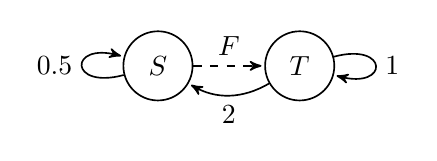
\begin{tikzpicture}[->,>=stealth',shorten >=1pt,auto,node distance=1.80cm,
		semithick]
		\tikzstyle{every state}=[fill=white,draw=black,text=black]
		
		\node[state] (s0)                    {$S$};
		\node[state]         (sn) [right of=s0]       {$T$};
		\path[->, dashed]
		(s0) edge 	node {$F$} (sn);
		\path[->]
		(s0) edge [loop left]	node {0.5} (s0)
			
		(sn) edge [bend left]	node {2} (s0)
		edge [loop right]	node {1} (sn);			
		\end{tikzpicture}
		\caption{Model of a simple ACTMC $\mathcal{A}$, $F$ is a non-Markovian distribution.}
		\label{fig:simple_actmc}
	\end{figure}
	
	\begin{figure}
		\centering
		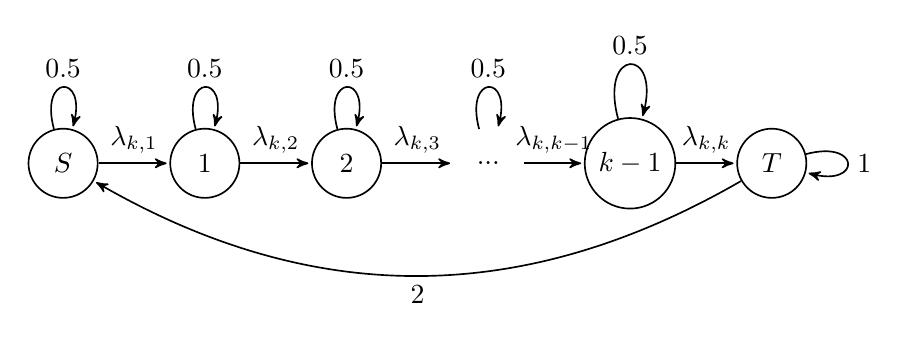
\begin{tikzpicture}[->,>=stealth',shorten >=1pt,auto,node distance=1.80cm,
		semithick]
		\tikzstyle{every state}=[fill=white,draw=black,text=black]
		
		\node[state] (s0)                    {$S$};
		\node[state]         (s1) [right of=s0] {$1$};
		\node[state]         (s2) [right of=s1] {$2$};
		\node[state,draw=none]         (s4) [right of=s2]       {$...$};
		\node[state]         (sw) [right of=s4,fill=white,text=black]       {$k-1$};
		\node[state]         (sn) [right of=sw]       {$T$};
		
		
		
		\path[->]  
		(s0) edge	node {$\lambda_{k,1}$} (s1)
			edge [loop above]	node {0.5} (s0);
		\path[->]
	
		[->]
		(s1) edge	node {$\lambda_{k,2}$} (s2)
			edge [loop above]	node {0.5} (s1);
		\path[->]
	
	
		(s2) edge   node {$\lambda_{k,3}$} (s4)
			edge [loop above]	node {0.5} (s2);
		\path[->]
	
	
		(s4) edge   node {$\lambda_{k,k-1}$} (sw)
			edge [loop above]	node {0.5} (s4);
		\path[->]
	
	
		(sw) edge   node {$\lambda_{k,k}$} (sn)
			edge [loop above]	node {0.5} (sw);
		\path[->]
		
		(sn) edge [bend left]	node {2} (s0)
		edge [loop right]	node {1} (sn);
		\end{tikzpicture}
		\caption{Model of a CTMC obtain by PH fitting of the ACTMC figure \ref{fig:simple_actmc}.}
		\label{fig:simple_ctmc}
	\end{figure}
In the case F is a Dirac of parameter $t$, we can set $\lambda_{i,k} = k/t$ for all $i$.
In order to deduce the SSP of Figure \ref{fig:simple_actmc}, we will add the SSP of Figure \ref{fig:simple_ctmc}. The sum of the states $\{A,1,2,...,k-1\}$ will be the probability of the state $S$ in the ACTMC. The probability of the state $T$ in the ACTMC will be the probability of the state $T$ in the CTMC. In Fact, Erlang($k$,$k/t$) is converging to Dirac($t$). This result is the key to Phase-Type deterministic timeouts.


	\section{Experimental evaluation}
	\label{experimetal_evaluation}
	
	\begin{figure}[H]
		\centering
		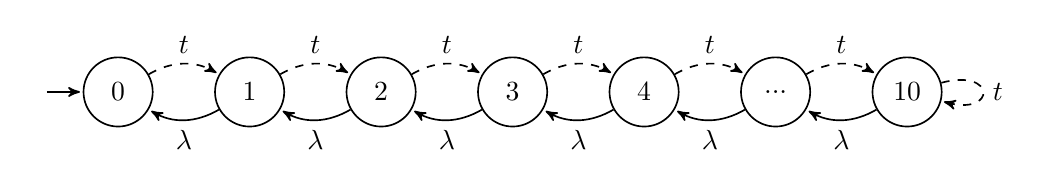
\begin{tikzpicture}[->,>=stealth',shorten >=1pt,auto,node distance=1.67cm,
		semithick]
		\tikzstyle{every state}=[fill=white,draw=black,text=black]
		
		\node[initial, initial text ={},state] (s0)                    {$0$};
		\node[state]         (s1) [right of=s0] {$1$};
		\node[state]         (s2) [right of=s1] {$2$};
		\node[state]         (s3) [right of=s2] {$3$};
		\node[state]         (s4) [right of=s3]       {$4$};
		\node[state]         (sw) [right of=s4,fill=white,text=black]       {...};
		\node[state]         (sn) [right of=sw]       {$10$};
		
		
		
		\path[->, dashed]  
		(s0) edge [bend left]             node {$t$} (s1);
		\path[->]
		(s1) edge [bend left] node {$\lambda$} (s0);
		\path[->, dashed]
		(s1) edge  [bend left]            node {$t$} (s2);
		\path[->]
		(s2) edge [bend left]             node {$\lambda$} (s1);
		\path[->, dashed]
		(s2) edge [bend left]  node {$t$} (s3);
		\path[->]
		(s3) edge [bend left]              node {$\lambda$} (s2);
		\path[->, dashed]
		(s3) edge [bend left]  node {$t$} (s4);
		\path[->]
		(s4) edge [bend left]             node {$\lambda$} (s3);
		\path[->, dashed]
		(s4) edge [bend left]  node {$t$} (sw);
		\path[->]
		(sw) edge [bend left]             node {$\lambda$} (s4);
		\path[->, dashed]
		(sw) edge [bend left]  node {$t$} (sn);
		\path[->]
		(sn) edge [bend left]             node {$\lambda$} (sw);
		\path[->, dashed]
		(sn) edge [loop right]  node {$t$} (sn);
		\end{tikzpicture}
		\caption{Model of a D/M/1/10 queue with production timeout $t = 0.1$ and service rate $\lambda = \frac{ln(2)}{t} \approx 6.931471805599453094$. The deterministic arrival event does not reset when the exponential service event occurs.}
		\label{fig:D/M/1/10}
	\end{figure}
	
	We have chosen to model a D/M/1/10 queue (deterministic arrivals, exponentially distributed service, single server, capacity of 10) as shown in Figure \ref{fig:D/M/1/10}. The deterministic arrivals are approximated by a phase-type distribution, so the model remains a CTMC and can be analyzed by PRISM. The PRISM model we used is shown in Figure \ref{fig:D/M/1/10_PRISM}.
	We computed the steady-state distribution with various values of PRISM termination epsilon $\epsilon$ and the number of phases $k$.
	
	\begin{figure}[H]
		\begin{lstlisting}
		ctmc
		
		const int k;
		const int qCapacity = 10;
		const double timeout = 0.1;
		const double lambda = 6.931471805599453094;
		
		module main
		
		qSize : [0..qCapacity] init 0;
		
		[produce] (qSize <= qCapacity) -> (qSize' = min(qSize+1,qCapacity));
		[consume] (qSize > 0) -> lambda: (qSize' = qSize - 1);
		
		endmodule
		
		module trigger
		
		i : [1..k+1];
		
		[] i < k -> k/timeout : (i'=i+1);
		[produce] i = k -> k/timeout : (i'=1);
		
		endmodule
		\end{lstlisting}
		\caption{PRISM CTMC model of the D/M/1/10 queue as shown in Figure \ref{fig:D/M/1/10} with a phase-type distribution approximating the arrival timeout. The phase-type module \emph{trigger} is used as suggested on the \href{http://www.prismmodelchecker.org/manual/FrequentlyAskedQuestions/PRISMModelling}{PRISM website}. Phase-type parameter $k$ represents the number of phases. Increasing $k$ should improve the approximation of the timeout. }
		\label{fig:D/M/1/10_PRISM}
	\end{figure}
	
	%\pagebreak
	\subsection{Obtaining precise results}
	\label{reference}
	
	%%%	In order to obtain some steady-state probabilities of reference to compare precision of different tools and engines, we computed the same steady-state probabilities two different ways. The first one is the phase type fitting method described as above (ref to the first page). The second one is by using our PRISM ACTMC implementation with precise termination epsilon.
	%%%	 the computation  results are quite similar as shown in picture citation
	
	%%%	 put picture diff_per_stqte 
	%%%	 explain picture
	
	%%% little conclusion: we can from now trust the event model as a reference 
	
	%%	 In order to compare the precision of the results obtained by the experiments, a trustworthy high-precision reference is needed. To achieve this, we used our own PRISM ACTMC implementation, which is capable of analyzing the given model directly without phase-type fitting. Using our implementation, we have computed the steady-state probabilities for very precise termination epsilon $\epsilon = 10^{-20}$ and compared it to the steady-state probabilities obtained by PRISM CTMC with phase-type fitting for $\epsilon = 10^{-16}$ and $k = 1000000$. As shown in Figure \ref{fig:diff_storm_dynamic}, the differences between the computations are smaller than $10^6$. Under the hypothesis that the true result is closer to the result obtained from PRISM ACTMC than to the result obtained from Storm, we can conclude that the PRISM ACTMC can serve as reference with precision at least $10^{-6}$.%%
	
	In order to compare the precision of the results obtained by the experiments, a trustworthy high-precision reference is needed. To achieve this ground truth, we have modeled the given D/M/1/10 queue in Oris \cite{Bucci2010}. The steady-state distribution obtained by Oris equals the steady-state distribution obtained by our GSMP PRISM with termination epsilon $10^{-20}$ implementation up to at least 14 digits. Hence, our tool can be considered a trustworthy reference with precision of $10^{-14}$.
	
	In the following, we will compare the distance between the SSP of the different approaches. This distance is the largest absolute difference between the distribution and the one computed with GSMP PRISM with termination epsilon $10^{-20}$.

	\subsection{Default parameters}
	\label{default_absolute}
	
	First, we used the PRISM with its default parameter setting. The results for increasing $k$ are shown in Figure \ref{fig:distance_constant_standard_constant_kappa}. The obtained results are arguably insufficient. Increasing $k$ does little to improve the precision, and only up to about $k \leq 50$, at which point increasing $k$ further starts making the precision worse. The reason is that PRISM has a parameter "Termination epsilon" that is set to $10^{-6}$ by default. This parameter specifies the precision of certain computation steps of PRISM. Increasing $k$ rises the number of states, hence the number of computation steps. This yields to increasing the overall error. 
	
	The last curve "PRISM ACTMC" is our version of PRISM. The absolute termination epsilon used is the same, $10^{-6}$. We observe that the error is closed to epsilon. Which is what we expect from a precision setting.
	
	\begin{figure}[H]
		\begin{center}
			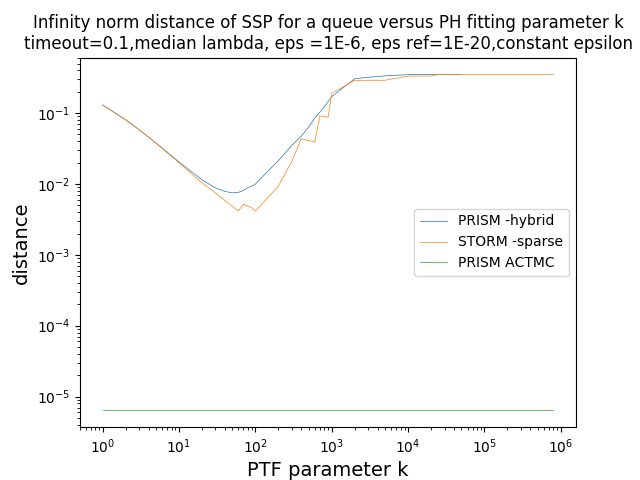
\includegraphics[trim=0.3cm 0cm 0cm 1.35cm,width=10cm, clip]{../picture/New_model/1E-6/distance_constant_1E-6.png}
		\end{center}
		\caption{Maximum distance (infinity norm) of the steady-state probabilities from the reference high-precision ACTMC ($10^{-20}$) against various values of $k$ for default absolute termination epsilon $\epsilon = 10^{-6}$. ACTMC results for $\epsilon = 10^{-6}$ are also compared to the reference.}
		\label{fig:distance_constant_standard_constant_kappa}
	\end{figure}
	
	%\pagebreak
	\subsection{Lowering absolute termination epsilon to $\epsilon = 10^{-10}$}
	\label{lowering}
	
	For much lower $\epsilon = 10^{-10}$, the precision of the result improves. However, for higher $k$ the precision continues to deteriorate like in Section \ref{default_absolute}. The results are shown in Figure \ref{fig:distance_constant_1E-10_constant_kappa}.
	Lowering the absolute termination increase the range of the PH parameter $k$ where the results are better. But for higher $k$, the precision keeps degrading. We have to adjust the precision when changing $k$. 
	
	We observe once more that the error for the GSMP PRISM computation is in the range of the absolute termination epsilon.
	
	\begin{figure}[H]
		\begin{center}
			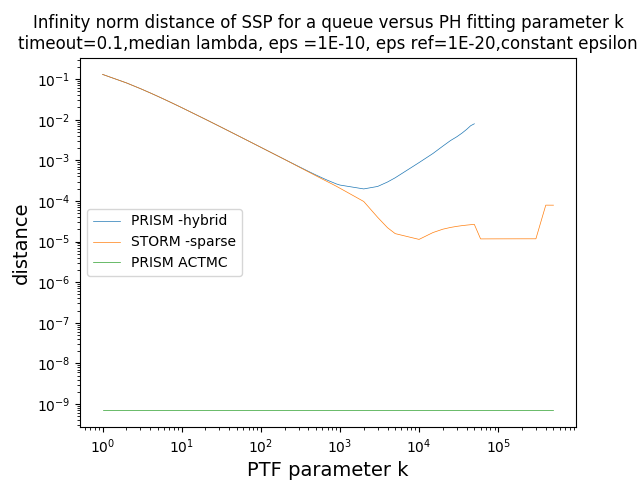
\includegraphics[trim=0.2cm 0cm 0cm 1.35cm,width=10cm, clip]{../picture/New_model/1E-10/distance_constant_1E-10.png}
		\end{center}
		\caption{Maximum distance (infinity norm) of the steady-state probabilities from the reference high-precision ACTMC ($10^{-20}$) against various values of $k$ for lowered absolute termination epsilon $\epsilon = 10^{-10}$. ACTMC results for $\epsilon = 10^{-10}$ are also compared to the reference.}
		\label{fig:distance_constant_1E-10_constant_kappa}
	\end{figure}
	
	%\pagebreak
	\subsection{Adjusting epsilon according to $k$}
	\label{adjusting}
	
	Since increasing $k$ increases the amount of phases (intermediate states) and each phase may have error up to $\epsilon$, the actual potential error for each state of the queue is $\epsilon \cdot k$. To compensate for this, we devise a simple formula
	$$\epsilon^{'} = \frac{\epsilon}{k}$$
	where $\epsilon^{'}$ is the adjusted epsilon that should be given to PRISM if precision $\epsilon$ is desired for $k$ phases.
	Using adjusted epsilon, the results get significantly better, as shown in Figure \ref{fig:distance_dynamic_1E-10_constant_kappa}. What's more, the phase-type fitting results now seem to converge towards the reference steadily as $k$ increases. This indicates that this approach is correct, and that our ground truth is correct.
	
	\begin{figure}[H]
		\begin{center}
			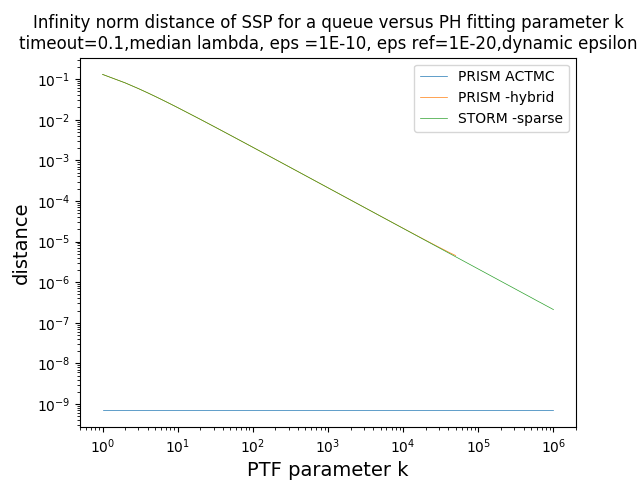
\includegraphics[trim=0.2cm 0cm 0cm 1.35cm,width=10cm, clip]{../picture/New_model/1E-10/distance_dynamic_1E-10.png}
		\end{center}
		\caption{Maximum distance (infinity norm) of the steady-state probabilities from the reference high-precision ACTMC ($10^{-20}$) against various values of $k$ for lowered and adjusted absolute termination epsilon $\epsilon = 10^{-10}$. ACTMC results for $\epsilon = 10^{-10}$ are also compared to the reference.}
		\label{fig:distance_dynamic_1E-10_constant_kappa}
	\end{figure}
	
	\subsection{Required computation time to obtain precise results}
	\label{computation_time}
	
	Although we have shown it is possible to obtain relatively precise results using phase-type distributions, the precision comes at a rather steep cost in computation time. This is shown in Figure \ref{fig:performance_dynamic}. Note that even though Storm is one of the fastest available tool, it still struggles to deliver good precision within reasonable time. All the computations ran on the same virtual machine under same conditions\footnote{Running in a virtual machine might have reduced the performance. The virtual machine we used is available at the \href{http://www.stormchecker.org/documentation/vm/vm.html}{Storm website}.}.
	
	\begin{figure}
		\begin{center}
			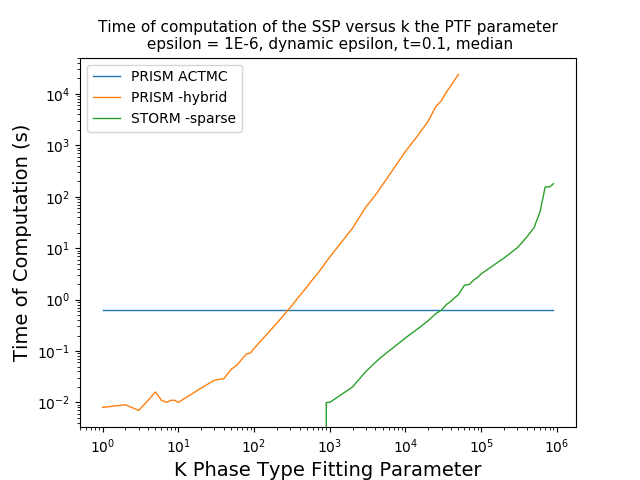
\includegraphics[trim=0.2cm 0cm 0cm 1.35cm,width=10cm, clip]{../picture/New_model/1E-6/performance_dynamic.png}
		\end{center}
		\caption{Time of computation in seconds of the steady-state probabilities against various values of $k$ for lowered and adjusted absolute termination epsilon $\epsilon = 10^{-10}$, i.e. corresponding to the data shown in Figure \ref{fig:distance_dynamic_1E-10_constant_kappa}. The computation of our PRISM ACTMC is constant in regards to $k$ because it does not use phase-type fitting. }
		\label{fig:performance_dynamic}
	\end{figure}
	
	\subsection{Another Model : firstRejuvenation}
	The firstRejuvenation model \cite{German:2000:PAC:518204} is originally a Stochastic Petri Net (SPN). I took it from a benchmark \cite{benchmark} made for evaluating fd-PRISM which is another version of Prism. The SPN graph is available in annexe, Figure \ref{fig:SPN_firstRejuvenation}. This model represent some production system that can be degraded with time (exponentially distributed). When the system is degraded, it can fail and has to be repaired. In the same time the system reset at every tic of a clock which put the system in his original state. 
	
	We can observe similar results in terms of lack of precision on another model Figure \ref{fig:fr_1E-10_constant}. The precision must also depend on the PH fitting parameter $k$ in this model. Here we went through difficulties related to the methods used by the engine in Prism. The Power method for computing SSP uses different iterations which are matrix multiplication. The number of iteration will strongly depend on the model and its parameter like timeouts and rates. In the First Rejuvenation model The convergence for the power method is really slow and the number of iteration required is important. In the queue, 100 000 000 iterations was enough to compute the SSP, but here the number of iteration prevent us to compute the SSP for k greater than 1000 with reasonable precision.
	
	The results of computation are given in the Figure \ref{fig:fr_1E-10_constant}. The orange curve is the error versus the number of phase $k$. The precision setting of the computation is $10^{-10}$ but the error is much bigger (at least $10^{-3}$). This error can be related to the theoretical approximation error of the PH fitting, but also the error of computation of the engine.
	\begin{figure}[H]
		\begin{center}
			\includegraphics[trim=0.2cm 0cm 0cm 1.35cm,width=10cm, clip]{../picture/firstRejuvenation/distance_1E-10_constant.png}
		\end{center}
		\caption{Maximum distance (infinity norm) of the steady-state probabilities from the reference high-precision ACTMC ($10^{-20}$) against various values of $k$ for lowered and adjusted absolute termination epsilon $\epsilon = 10^{-10}$. ACTMC results for $\epsilon = 10^{-10}$ are also compared to the reference.}
		\label{fig:fr_1E-10_constant}
	\end{figure}
	
	%\pagebreak
	\section{Conclusion}
	
	
%	CHANGE THIS
	
	We have presented a reliable method for high-precision analysis of PRISM CTMC models with phase-type distributions, that is, adjusting the termination epsilon by the number of phases. However, the large number of phases drastically increases the computation time.
	
	Using the default setting of precision when doing PH fitting is not reliable at all. The relation between the experimental precision and the parameter of the model is not trivial. We have presented a sufficient condition to increased the precision while increasing the number of phases. 
	
	For better performance, we suggest usage of more specialized tools that can deal with non-Markovian distributions directly, without phase-type fitting. Our PRISM ACTMC extension \footnote{Our PRISM ACTMC extension is not fully completed yet and lacks optimization. It will be officially released later, but early development version is available at \href{https://github.com/VojtechRehak/prism-gsmp}{https://github.com/VojtechRehak/prism-gsmp}.} has delivered results with sufficient precision a lot faster.
	
	This experimental statement strengthens the conjecture that further heuristics can increase the efficiency of an analysis with a non-Markovian distributions\cite{DBLP:journals/corr/KorenciakKR14}. To some extent GSMP-PRISM is challenging the PH fitting approach. Hence it could be interesting to compare the efficiency of GSMP-PRISM with the analysis of SPN with the tool Oris.
	
\subsubsection*{Acknowledgements}
I would like to thank Vojtech Reh{\'{a}}k, which has been  my supervisor during this internship. Also, I thank M\'{a}rio Uhr\'{i}k for his assistance during this internship and our joint contributions and discussions. 

\iffalse
\subsection{A Subsection Sample}
Please note that the first paragraph of a section or subsection is
not indented. The first paragraph that follows a table, figure,
equation etc. does not need an indent, either.

Subsequent paragraphs, however, are indented.

\subsubsection{Sample Heading (Third Level)} Only two levels of
headings should be numbered. Lower level headings remain unnumbered;
they are formatted as run-in headings.

\paragraph{Sample Heading (Fourth Level)}
The contribution should contain no more than four levels of
headings. Table~\ref{tab1} gives a summary of all heading levels.

\begin{table}
\caption{Table captions should be placed above the
tables.}\label{tab1}
\begin{tabular}{|l|l|l|}
\hline
Heading level &  Example & Font size and style\\
\hline
Title (centered) &  {\Large\bfseries Lecture Notes} & 14 point, bold\\
1st-level heading &  {\large\bfseries 1 Introduction} & 12 point, bold\\
2nd-level heading & {\bfseries 2.1 Printing Area} & 10 point, bold\\
3rd-level heading & {\bfseries Run-in Heading in Bold.} Text follows & 10 point, bold\\
4th-level heading & {\itshape Lowest Level Heading.} Text follows & 10 point, italic\\
\hline
\end{tabular}
\end{table}


\noindent Displayed equations are centered and set on a separate
line.
\begin{equation}
x + y = z
\end{equation}
Please try to avoid rasterized images for line-art diagrams and
schemas. Whenever possible, use vector graphics instead (see
Fig.~\ref{fig1}).

\begin{figure}
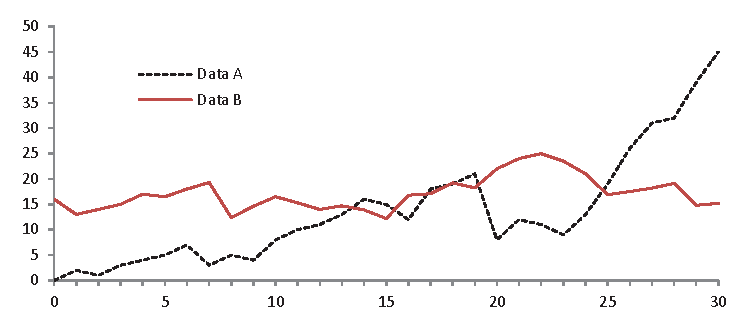
\includegraphics[width=\textwidth]{fig1.eps}
\caption{A figure caption is always placed below the illustration.
Please note that short captions are centered, while long ones are
justified by the macro package automatically.} \label{fig1}
\end{figure}

\begin{theorem}
This is a sample theorem. The run-in heading is set in bold, while
the following text appears in italics. Definitions, lemmas,
propositions, and corollaries are styled the same way.
\end{theorem}
%
% the environments 'definition', 'lemma', 'proposition', 'corollary',
% 'remark', and 'example' are defined in the LLNCS documentclass as well.
%
\begin{proof}
Proofs, examples, and remarks have the initial word in italics,
while the following text appears in normal font.
\end{proof}
For citations of references, we prefer the use of square brackets
and consecutive numbers. Citations using labels or the author/year
convention are also acceptable. The following bibliography provides
a sample reference list with entries for journal
articles~\cite{ref_article1}, an LNCS chapter~\cite{ref_lncs1}, a
book~\cite{ref_book1}, proceedings without editors~\cite{ref_proc1},
and a homepage~\cite{ref_url1}. Multiple citations are grouped
\cite{ref_article1,ref_lncs1,ref_book1},
\cite{ref_article1,ref_book1,ref_proc1,ref_url1}.
\section{Conclusion}
%
% ---- Bibliography ----
%
% BibTeX users should specify bibliography style 'splncs04'.
% References will then be sorted and formatted in the correct style.
%
% \bibliographystyle{splncs04}
% \bibliography{mybibliography}

\begin{thebibliography}{8}
\bibitem{ref_article1}
Author, F.: Article title. Journal \textbf{2}(5), 99--110 (2016)

\bibitem{ref_lncs1}
Author, F., Author, S.: Title of a proceedings paper. In: Editor,
F., Editor, S. (eds.) CONFERENCE 2016, LNCS, vol. 9999, pp. 1--13.
Springer, Heidelberg (2016). \doi{10.10007/1234567890}

\bibitem{ref_book1}
Author, F., Author, S., Author, T.: Book title. 2nd edn. Publisher,
Location (1999)

\bibitem{ref_proc1}
Author, A.-B.: Contribution title. In: 9th International Proceedings
on Proceedings, pp. 1--2. Publisher, Location (2010)

\bibitem{ref_url1}
LNCS Homepage, \url{http://www.springer.com/lncs}. Last accessed 4
Oct 2017

\end{thebibliography}
\fi
\section*{Annexe}
\printbibliography

	\begin{figure}[H]
		\begin{center}
			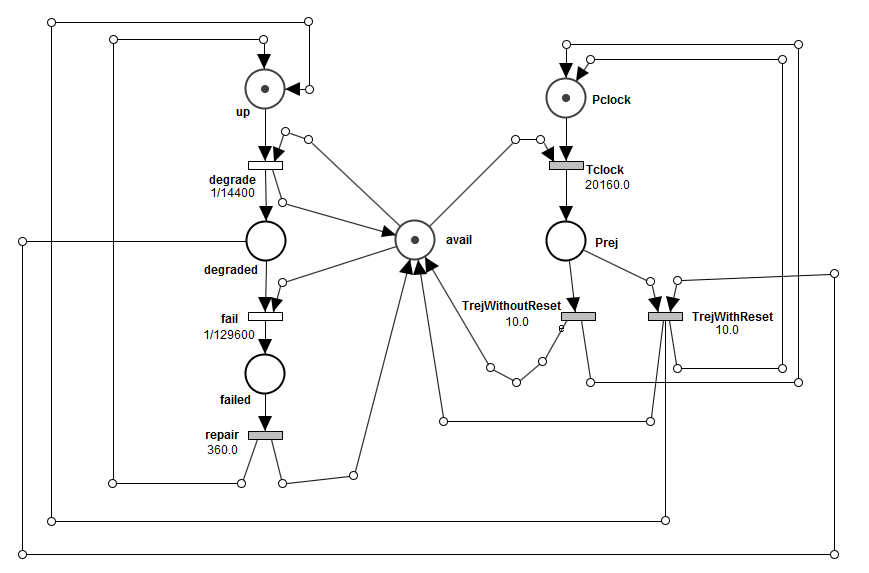
\includegraphics[,width=10cm, clip]{../../Model/benchmark/release/firstRejuvenation/firstRejuvenationPIC.png}
		\end{center}
		\caption{SPN model of firstRejuvenation. Grey transitions are deterministic (Dirac) transitions. White filled transitions are exponential transitions.}
		\label{fig:SPN_firstRejuvenation}
	\end{figure}
\end{document}
